\chapter{Introduction}
\label{ch:Introduction}

\section{General}

\subsection{Parkinson's Disease}

According to \cite{patients_medical_definition_2014}, Parkinson's disease (PD)\nomenclature{PD}{Parkinson's disease} is a progressive, neurodegenerative disease that occurs when the neurons within the brain responsible for producing the chemical dopamine become impaired or die. Dopamine is essential for the smooth control and coordination of the movement of voluntary muscle groups. Once approximately 80\% of the brain's dopamine producing cells no longer function, the symptoms of PD begin to appear. Parkinson's disease may be termed as a progressive movement disorder that is distinguished by marked slow movements, tremors, and unstable posture.

When attempting to voluntarily initiate the first step to begin walking, many patients with PD exhibit start hesitation and freezing, especially in advanced stages of the disease \cite{mancini_anticipatory_2009}. \cite{jacobs_knee_2009} states that freezing of gait (FoG)\nomenclature{FoG}{Freezing of Gait} is an episodic, brief inability to step that delays gait initiation or interrupts ongoing gait. FoG is often associated with an alternating shaking of the knees, clinically referred to as knee trembling or trembling in place. However, these clinical signs of balance or gait problems are not evident in early stages of the desease \cite{mancini_anticipatory_2009}.

\subsection{Anticipatory Postural Adjustments}

Immediately prior to step initiation, anticipatory postural adjustments (APAs) act to accelerate the centre of body mass (COM)\nomenclature{COM}{Centre of Mass} forward and laterally over the stance foot by moving the centre of pressure (COP)\nomenclature{COP}{Centre of Pressure} posteriorly and toward the stepping leg \cite{mancini_anticipatory_2009} (see figure \ref{fig:APAoverview}). The S1 period encompasses the uncoupling of the COP and COM as the COP displaces posteriorly and toward the intended stepping limb. During the subsequent S2 period, the COP moves mediolaterally toward the stance foot. Finally, during the S3 period the COP moves anteriorly under the stance foot.

\begin{figure}
	\centering
	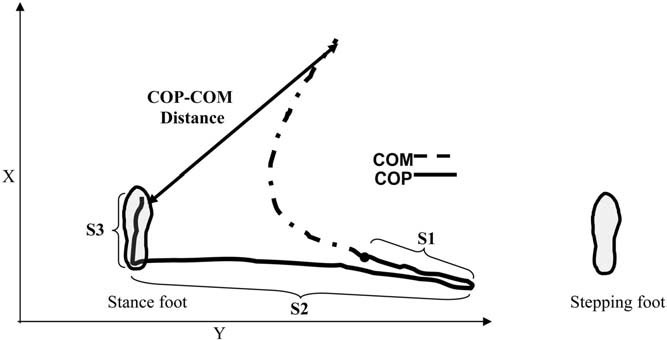
\epsfig{file=images/APA_overview, width=9cm}
	\caption{Overhead view of the path of the COP and COM during forward-oriented gait initiation when stepping with the right foot. The arrow represents the distance between the COP-COM \cite{hass_gait_2005-1}}
	\label{fig:APAoverview}
\end{figure}


\section{Motivation}

Advanced PD can increasingly diminish quality of life due to the fact that patients are dependent on help from other doing daily tasks. Early diagnosis of PD could 


\section{Goals}

The main goal was to build a classifier which is fed with data from both force plate and magnetic inertial measurement unit (MIMU)\nomenclature{MIMU}{Magnetic Intertial Measurement Unit} to distunguish between Parkinson patients and healthy subjects.


\section{State of the art}

There are several methods and devices to assess Parkinson's disease. The state of the art is presented below.

\subsection{Rating scales}

One commonly used rating scale is the Unified Parkinson’s Disease Rating Scale (UPDRS)\nomenclature{UPDRS}{Unified Parkinson’s Disease Rating Scale} which is a short test performed by a physician \cite{klerk_long-term_2009}. Another method is the Hoehn and Yahr scale (HY)\nomenclature{HY}{Hoehn and Yahr scale}. Strengths of the HY scale include its wide utilization and acceptance. Weaknesses include the scale's mixing of impairment and disability and its non-linearity \cite{goetz_movement_2004}. Both rating methods have disadvantages such as subjectivity, short observation periods and unfamiliarity of the environment.

\subsection{Instrumentation}

In addition to the named subjective rating scales there are different devices used to measure gait and assess it ojectively. All of them come with certain pros and cons. The following devices have been used:

\begin{itemize}

\item Electromyographs:

\item Force plates:

\item Inertial sensors:

\end{itemize}

\subsection{Calibration}

Different calibration methods are used...


\subsection{Classification}

Different classification methods are used...

